The Java front-end client is the main program that users will interact with to use the scanning utilities, which provides better visual representation of the utilities and logs, and increases usability compared to directly using the backend scripts.

\vspace{0.5cm}

\begin{figure}[h]
	\centering
	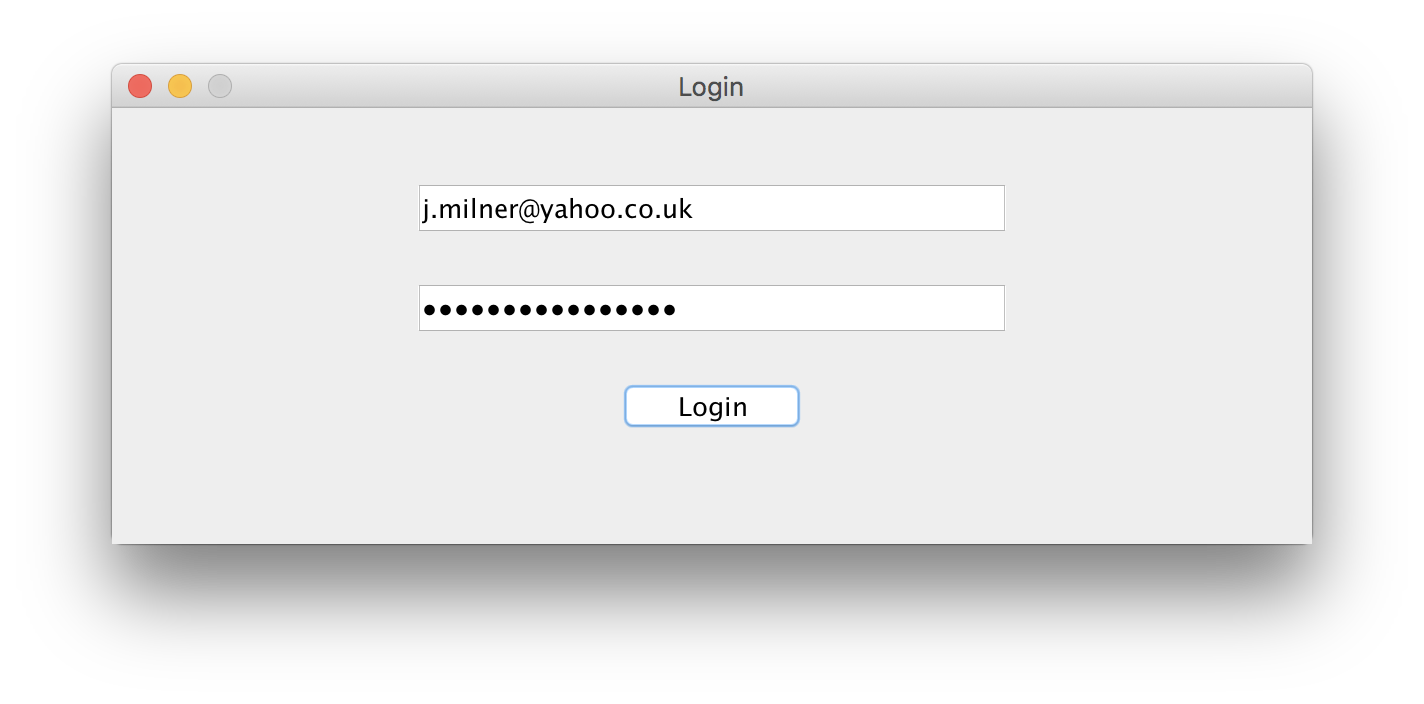
\includegraphics[width=1\linewidth]{img/login_screenshot.png}
	\caption{Login Window}
\end{figure}

As a user starts Miraihilate they will first be prompted to login to the program using the email and password shown in the setup program or from the admin user creation utility. The raw password entered by the user is then hashed using BCrypt to validate the hash stored with the email address in the database. If the two hashes are equal, then the user gains access to the functionality of Miraihilate's client interface.

\begin{figure}[h]
	\centering
	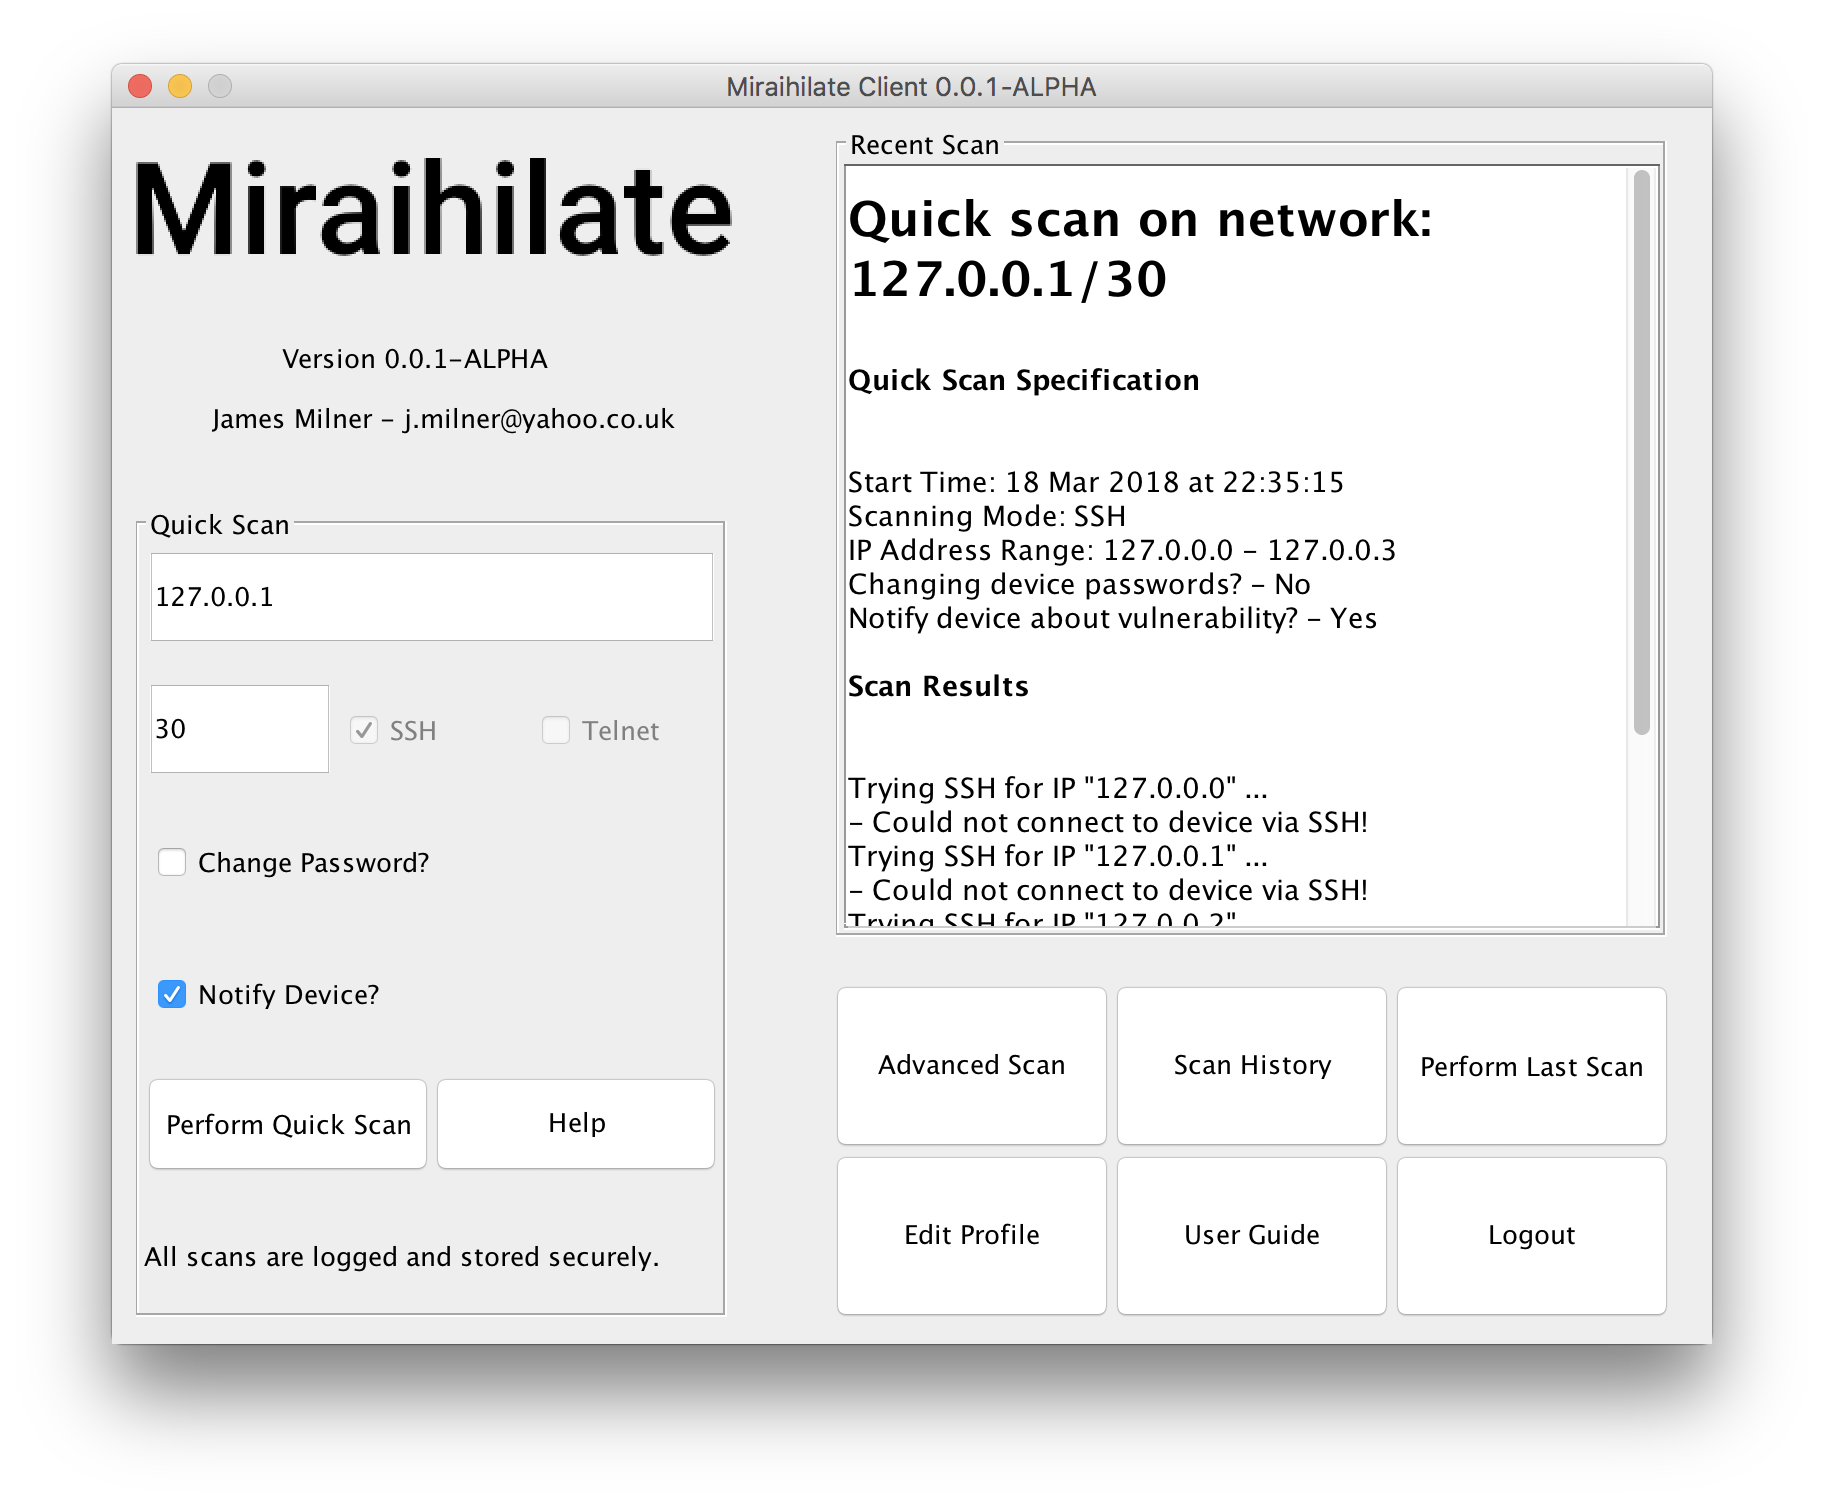
\includegraphics[width=1\linewidth]{img/client_iface_screenshot.png}
	\caption{Client Window}
\end{figure}

After successfully gaining access to the client, the user will be shown the main interface as shown in Figure 4.4. As seen in the image, the user will first see the quick scanning utility, a view for the log of their most recent scan and buttons for accessing other options the client offers.

\subsection{Quick Scanning}

The quick scanning utility provies users with the ability to initiate a simple scan on a network range. It provides minimal options for communicating with vulnerable devices and its primary aim is to check for vulnerable devices within the network. If a user does not remember how to operate the quick scanning utility they can either refer to the user guide, which is also accessible from the client interface, or they can click the help button from the quick scan panel. This will bring up a quick recap on what each of the fields for quick scanning mean and require, as shown in Figure 4.5.

\begin{figure}[h]
	\centering
	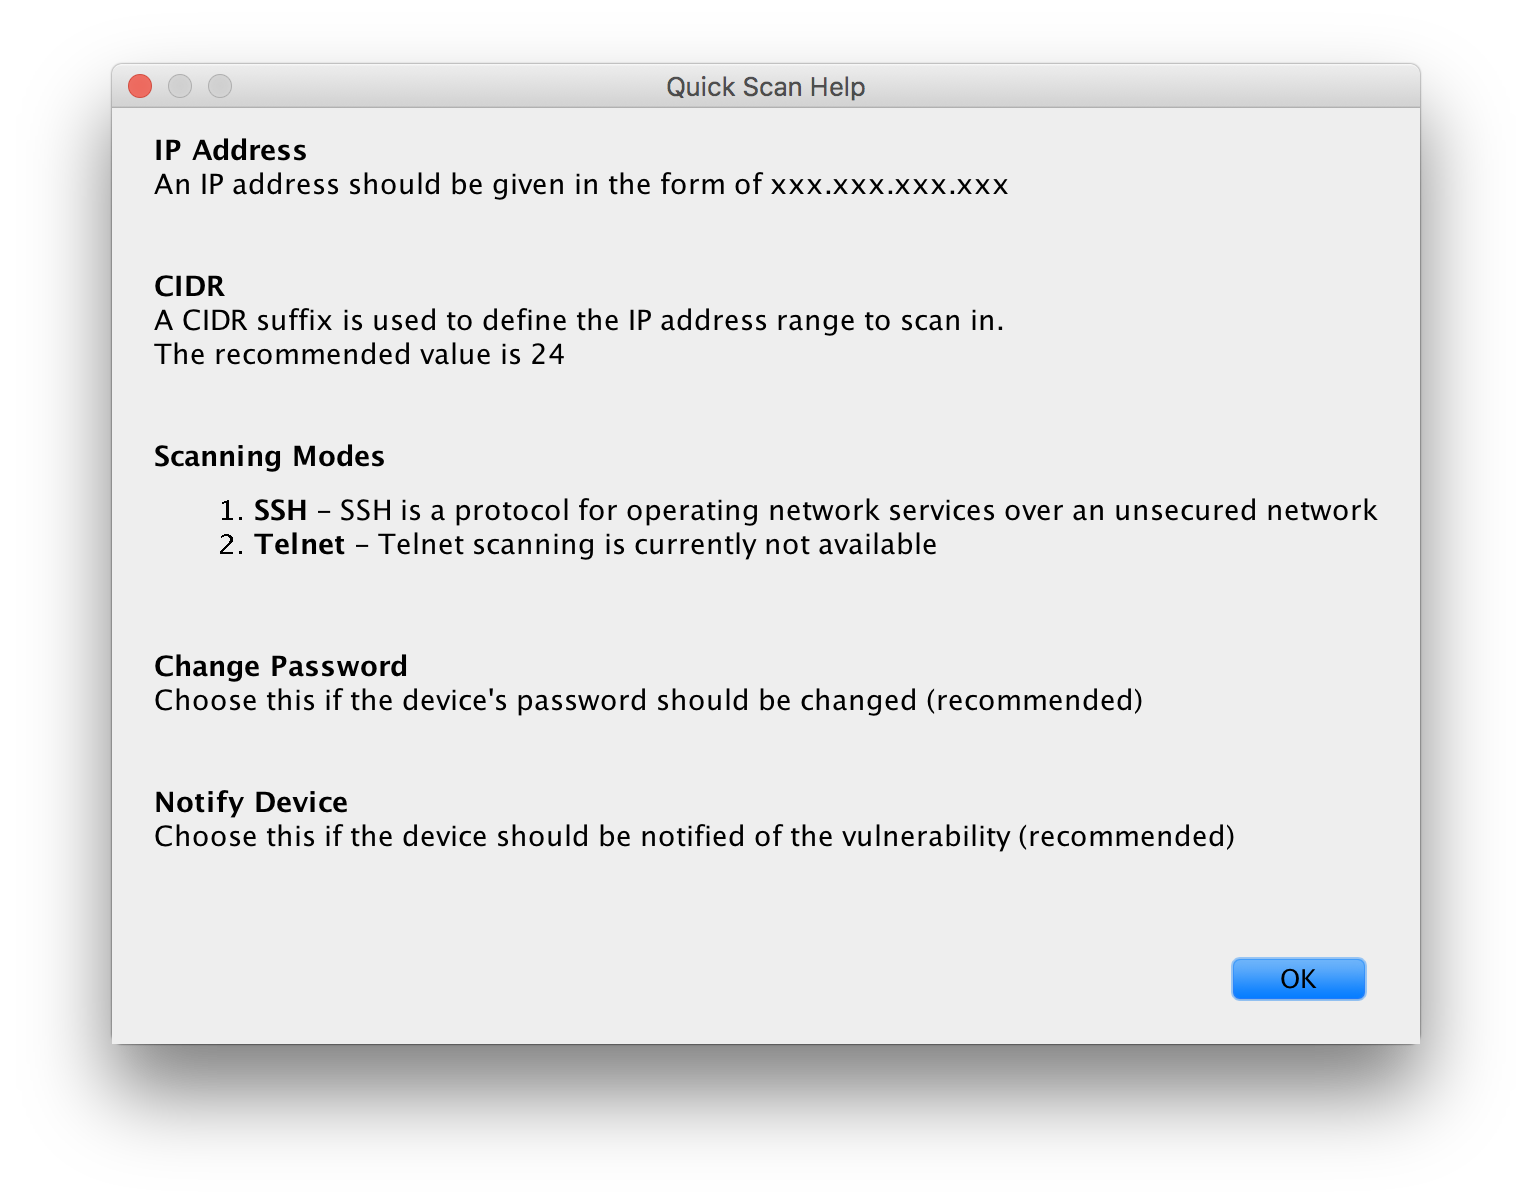
\includegraphics[width=1\linewidth]{img/quick_scan_help_screenshot.png}
	\caption{Quick Scan Help Window}
\end{figure}

\subsection{Viewing Scan Logs}

A user of Miraihilate will have two ways of viewing scan logs. The first is a fixed view of their most recent scan performed and the second being a list of all their scan logs to date. Originally, the scan log with stored as JSON data, but parsing JSON data into a text area on the client did not provide a good enough visual representaiton of the data. Therefore I decided to store the scan data as a HTML document and use a \textit{JEditorPane} to display HTML scan data from the database, so no parsing has to be done.

\vspace{2cm}

As seen in Figure 4.6, whilst viewing their scan history, users can select a scan item from list on the left panel to display its corresponding scan result in the view on the right. The client connects to the database to retrieve a list of the users scans in descending order, starting from the latest scan they have done. To support non-repudiation of scans, they cannot be deleted and scans are linked with the time they were performed and the UUID of the user who did the scan.

\vspace{0.5cm}

\begin{figure}[h]
	\begin{subfigure}[h]{0.5\linewidth}
		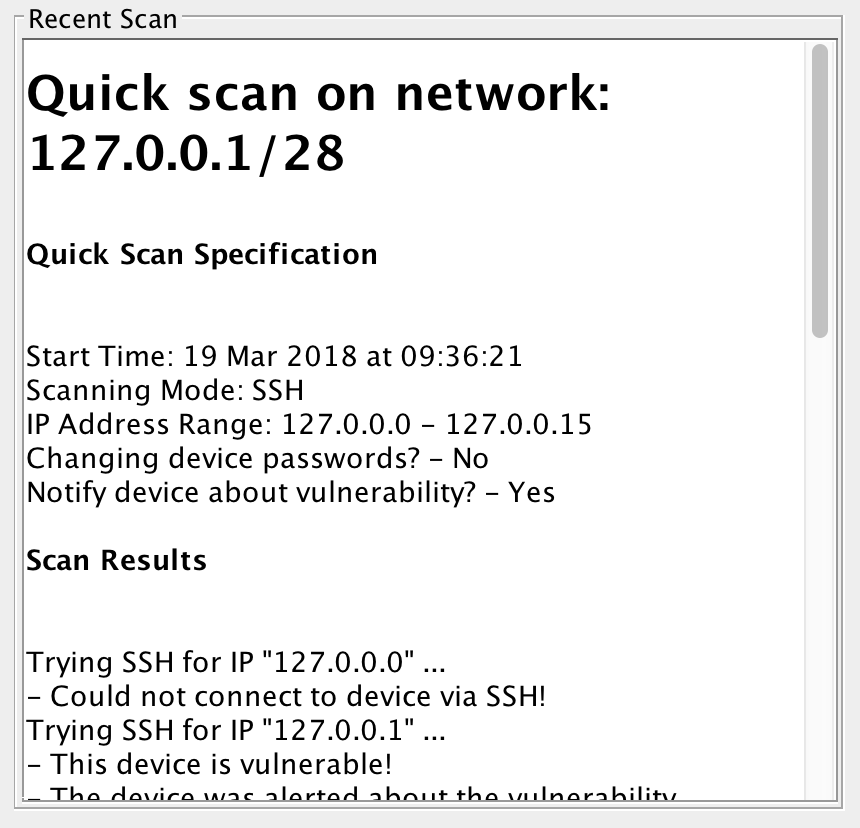
\includegraphics[width=\linewidth]{img/recent_scan_view_screenshot.png}
		\caption{Recent Scan View}
	\end{subfigure}
	\hfill
	\begin{subfigure}[h]{0.6\linewidth}
		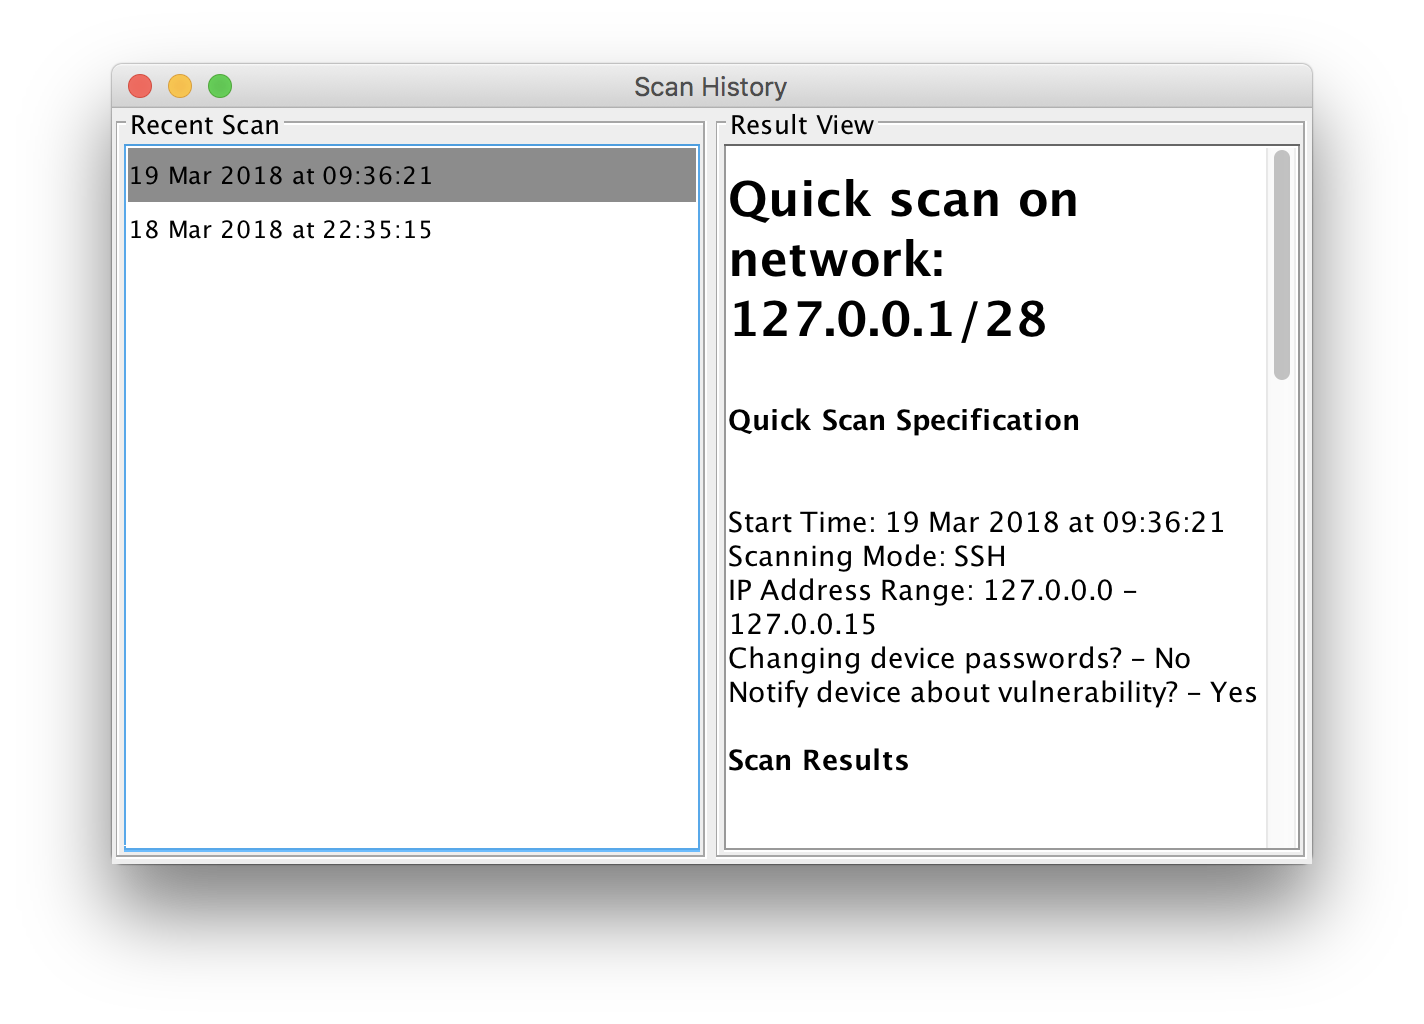
\includegraphics[width=\linewidth]{img/scan_history_screenshot.png}
		\caption{Scan History}
	\end{subfigure}
	\caption{Two Methods of Viewing Scan Logs}
\end{figure}

\clearpage

\subsection{Advanced Scanning}

\begin{figure}[h]
	\begin{center}
		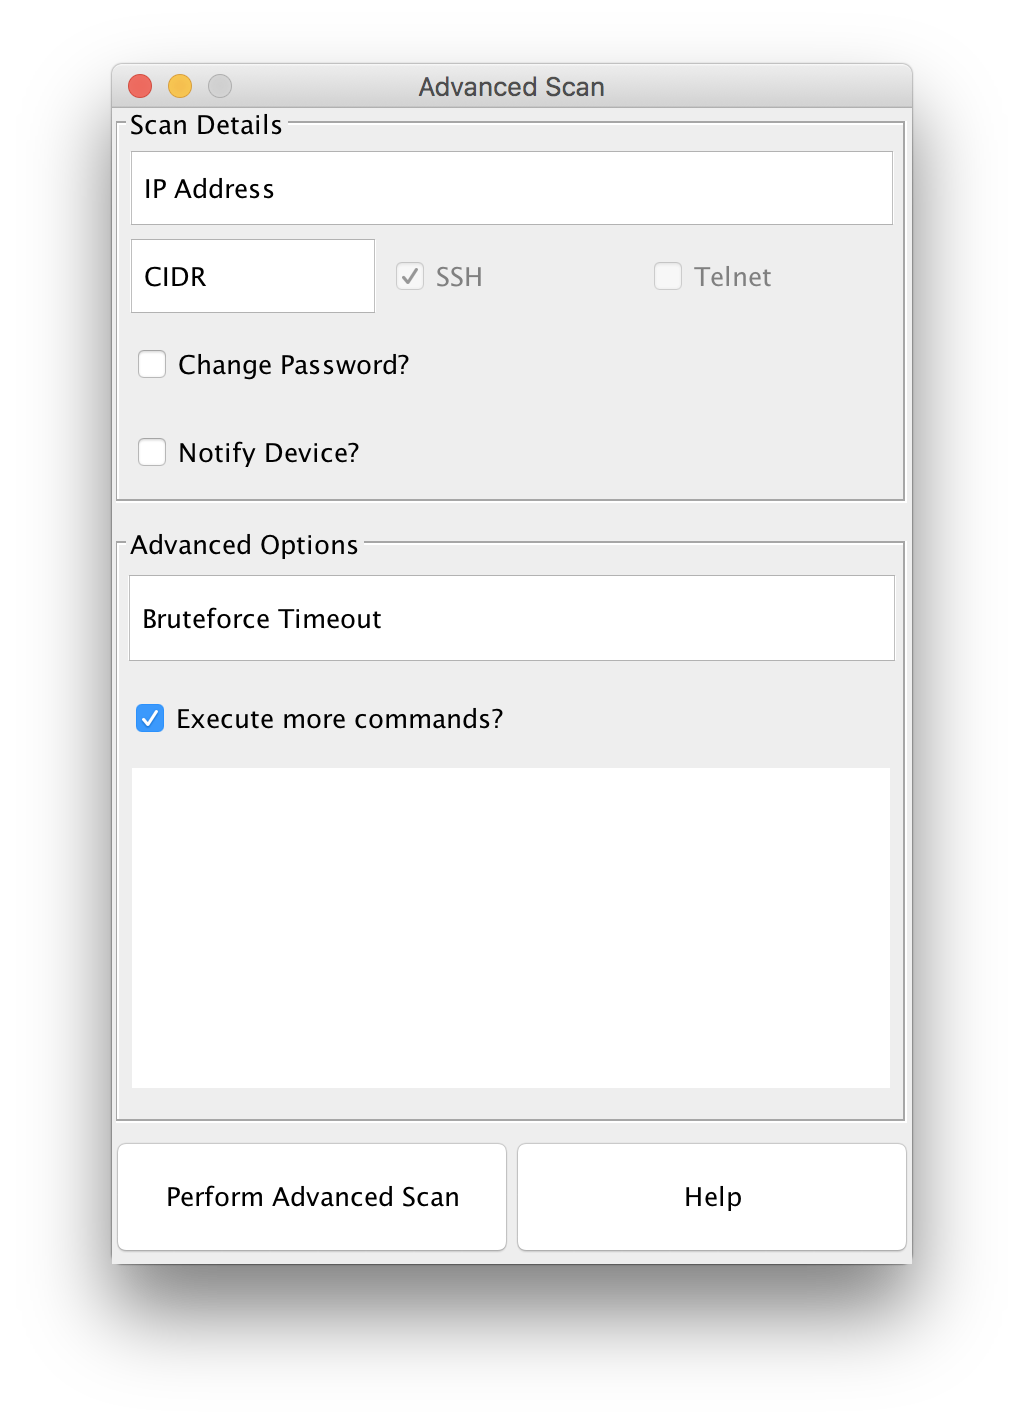
\includegraphics[width=0.5\textwidth]{img/advanced_scan_screenshot.png}
	\end{center}
	\caption{Advanced Scan Interface}
\end{figure}

As well as the quick scanning utility, the client interface also provides a window for advanced scanning. As shown in figure 4.7, the interface provides the same fields as a quick scan, with the added advanced options of choosing a timeout for the scans as well as the ability to provide extra commands to the device. These commands are not client-specific, but commands that can be executed via SSH to a unix-based operating system. Example commands include:

\begin{lstlisting}[language=bash]
	# Print system information
	uname -a
	# Download a shell file from a server and execute it
	wget http://<hostname> -O- | sh
	# Show who is logged on and what they are doing
	w
\end{lstlisting}
